\section{Stencil Applications}

\from{HiStencils begin}
For evaluating our two skeleton implementations, we study two stencil applications:
1) the Gaussian blur, a popular noise reduction technique in image processing, and
2) the Canny algorithm for detecting edges in images.
These two applications have different characteristics.
The Gaussian blur applies a single stencil computation, possibly iterated multiple times, for reducing the noise in images.
The Canny edge detection algorithm consists of a sequence of stencil operations which are applied once to obtain the final result.
For each application, we compare the performance of our MapOverlap and Stencil skeletons using an input image of size $4096 \times 3072$.

The measurements run on a Tesla S1070 computing system with $4$ GPUs, each providing $4$ GB of memory, accessing this memory with $102$ GB/s, and $240$ compute units per GPU running at $1.44$ GHz.
The GPUs are connected to the host system with a quad-core CPU (Intel E5520, $2.26$ GHz) and 12 GB of main memory.
$200$ runs were performed for each configuration and the average was calculated; to reduce measuring inaccuracy, the best and worst $5\%$ measurements were not considered. 
\from{HiStencils end}

\from{HiStencils begin}
\subsection{Gaussion Blur (HiStencils)}

\paragraph{Gaussian Blur with a single iteration}

\begin{figure}[tbp]
	\centering
	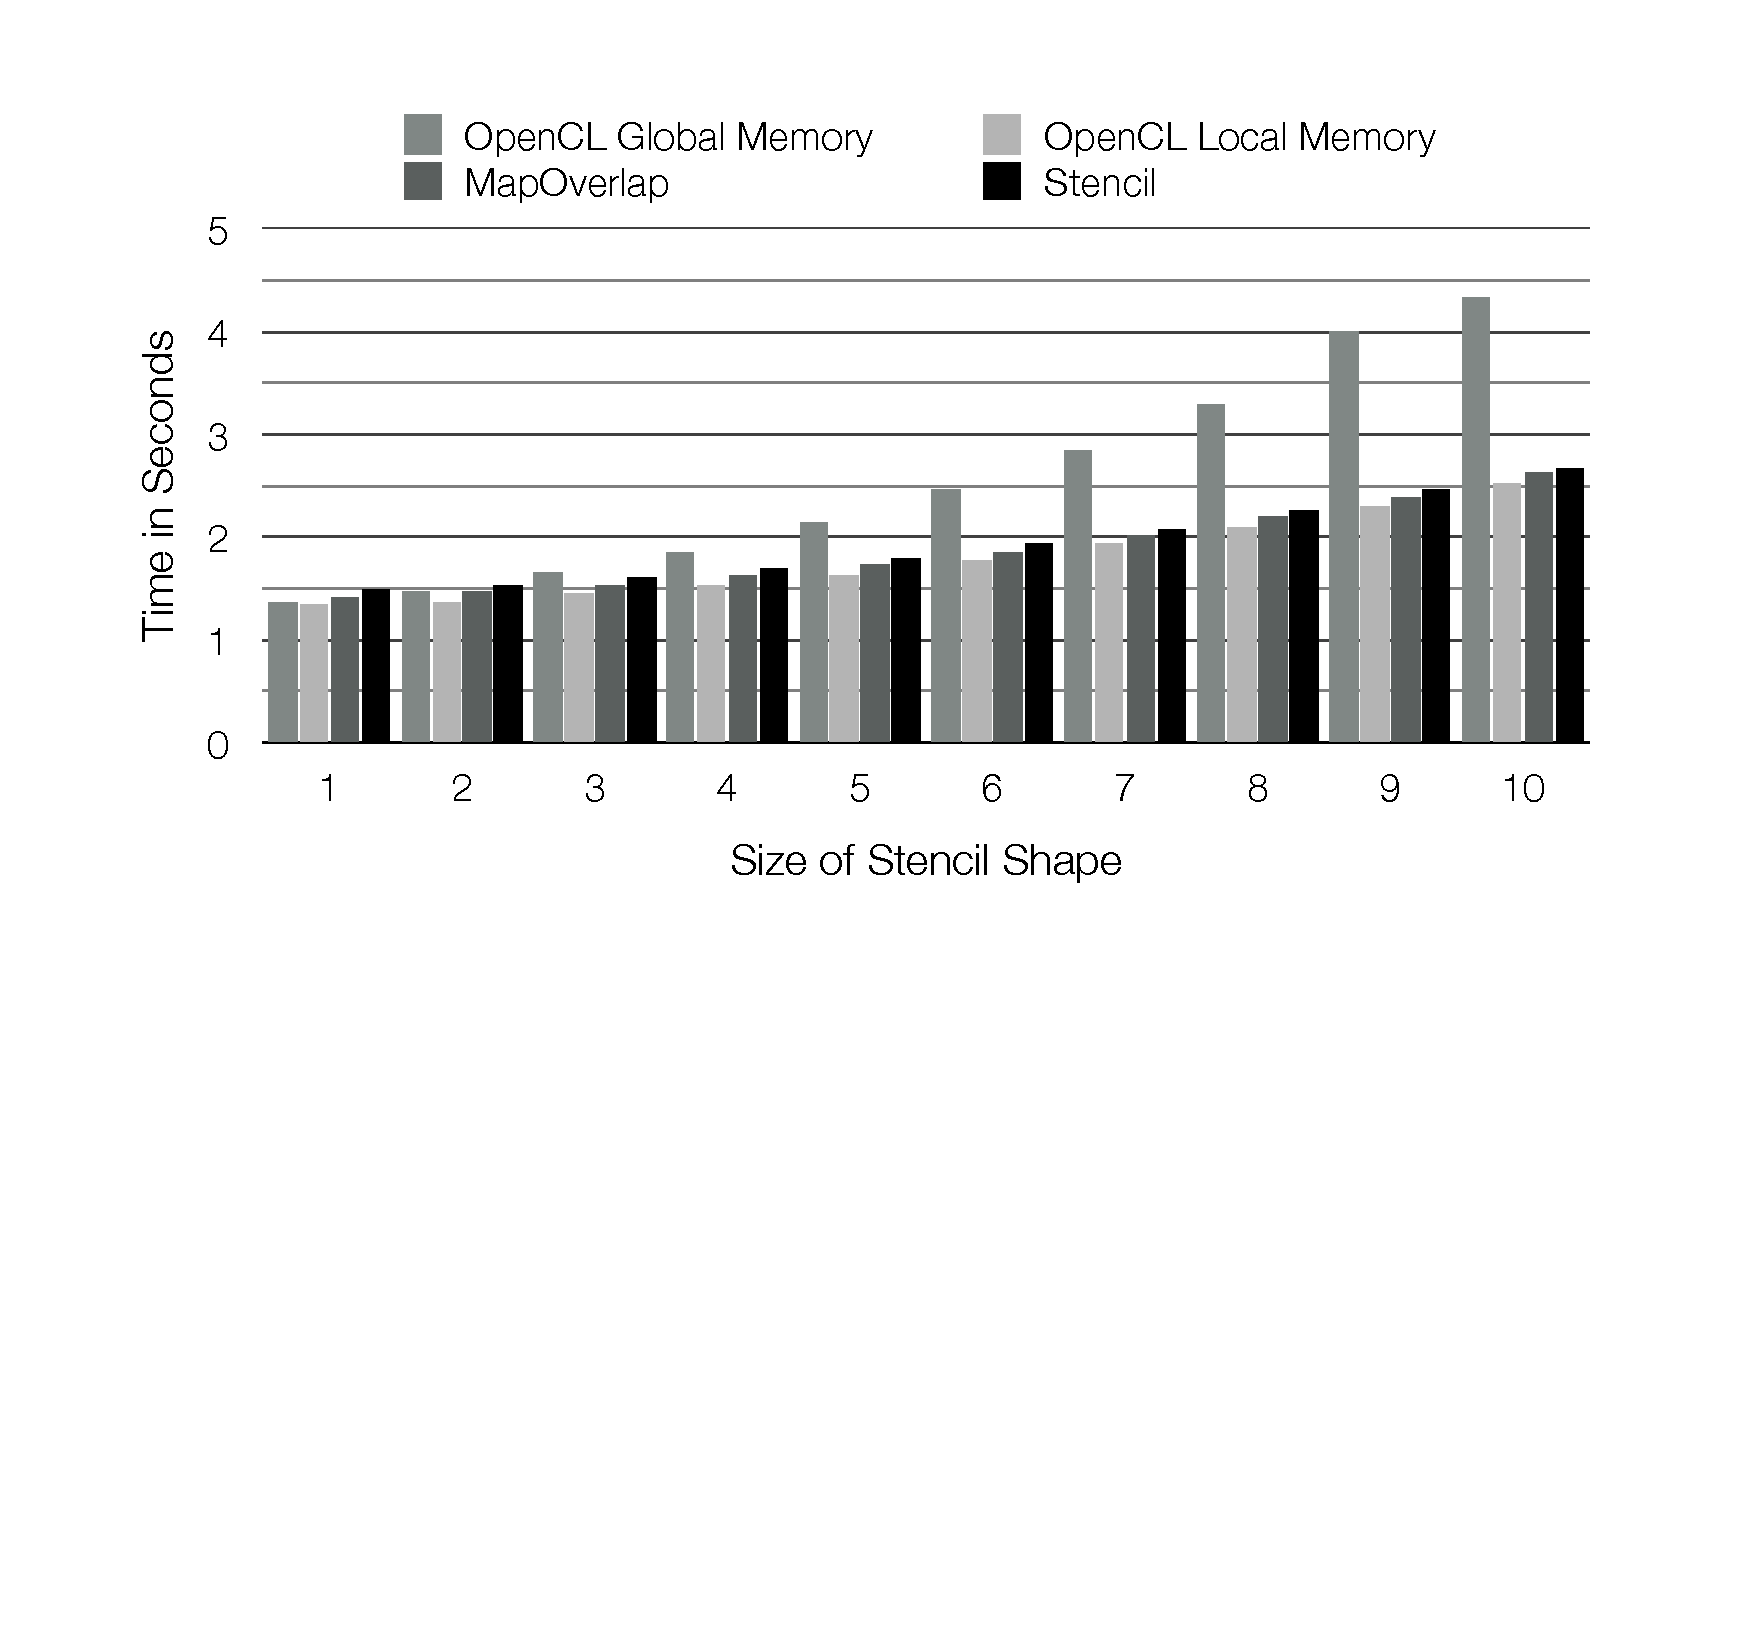
\includegraphics[width=\columnwidth]{HiStencils/GaussOpenCL.pdf}
	\caption{Runtime of the Gaussian blur using a na{\"i}ve OpenCL implementation with global memory, an OpenCL version using local memory and SkelCL's MapOverlap and Stencil skeletons.}
	\label{fig:gaussAbs}
\end{figure} 

Figure~\ref{fig:gaussAbs} shows the total runtime of the Gaussian blur using:
1) a na{\"i}ve OpenCL implementation using global memory,
2) an optimized OpenCL version using local memory, and
3) the MapOverlap, and
4) the Stencil skeletons for different sizes of stencil shape, correspondingly.
We observe that on larger stencil shape sizes, MapOverlap and Stencil outperform the na{\"i}ve OpenCL implementation by $65\%$ and $62\%$, respectively.
The optimized OpenCL version, which copies all necessary elements into local memory prior to calculation, is $5\%$ faster than MapOverlap and $10\%$ faster than Stencil for small stencil shapes.
When increasing the stencil shape size, this disadvantage is reduced to $3\%$ for MapOverlap and $5\%$ for Stencil with stencil shape's extent of $10$ in each direction.

As expected, the Stencil skeleton's implementation is slower for small stencil shapes than the MapOverlap skeleton's, up to $32\%$ slower for an stencil shape size of $1$. 
However, this disadvantage is reduced to $4.2\%$ for an stencil shape size of $5$ and becoming negligible for bigger stencil shape sizes.
Due to the increased branching in Stencil's kernel function, one might expect a worse runtime for the Stencil skeleton. 
As the ratio of copying into local memory decreases in comparison to the number of calculations when enlarging the stencil shape's extents, the Stencil skeleton kernel function's runtime converges to the MapOverlap skeleton's.
The Stencil skeleton's disadvantage is also due to its ability to manage multiple stencil shapes and explicitly support the use of iterations.
While both features are not used in this use case, they incur some overhead for the Stencil skeleton as compared to the MapOverlap skeleton for simple stencil computations.

\begin{figure}[tbp]
	\centering
	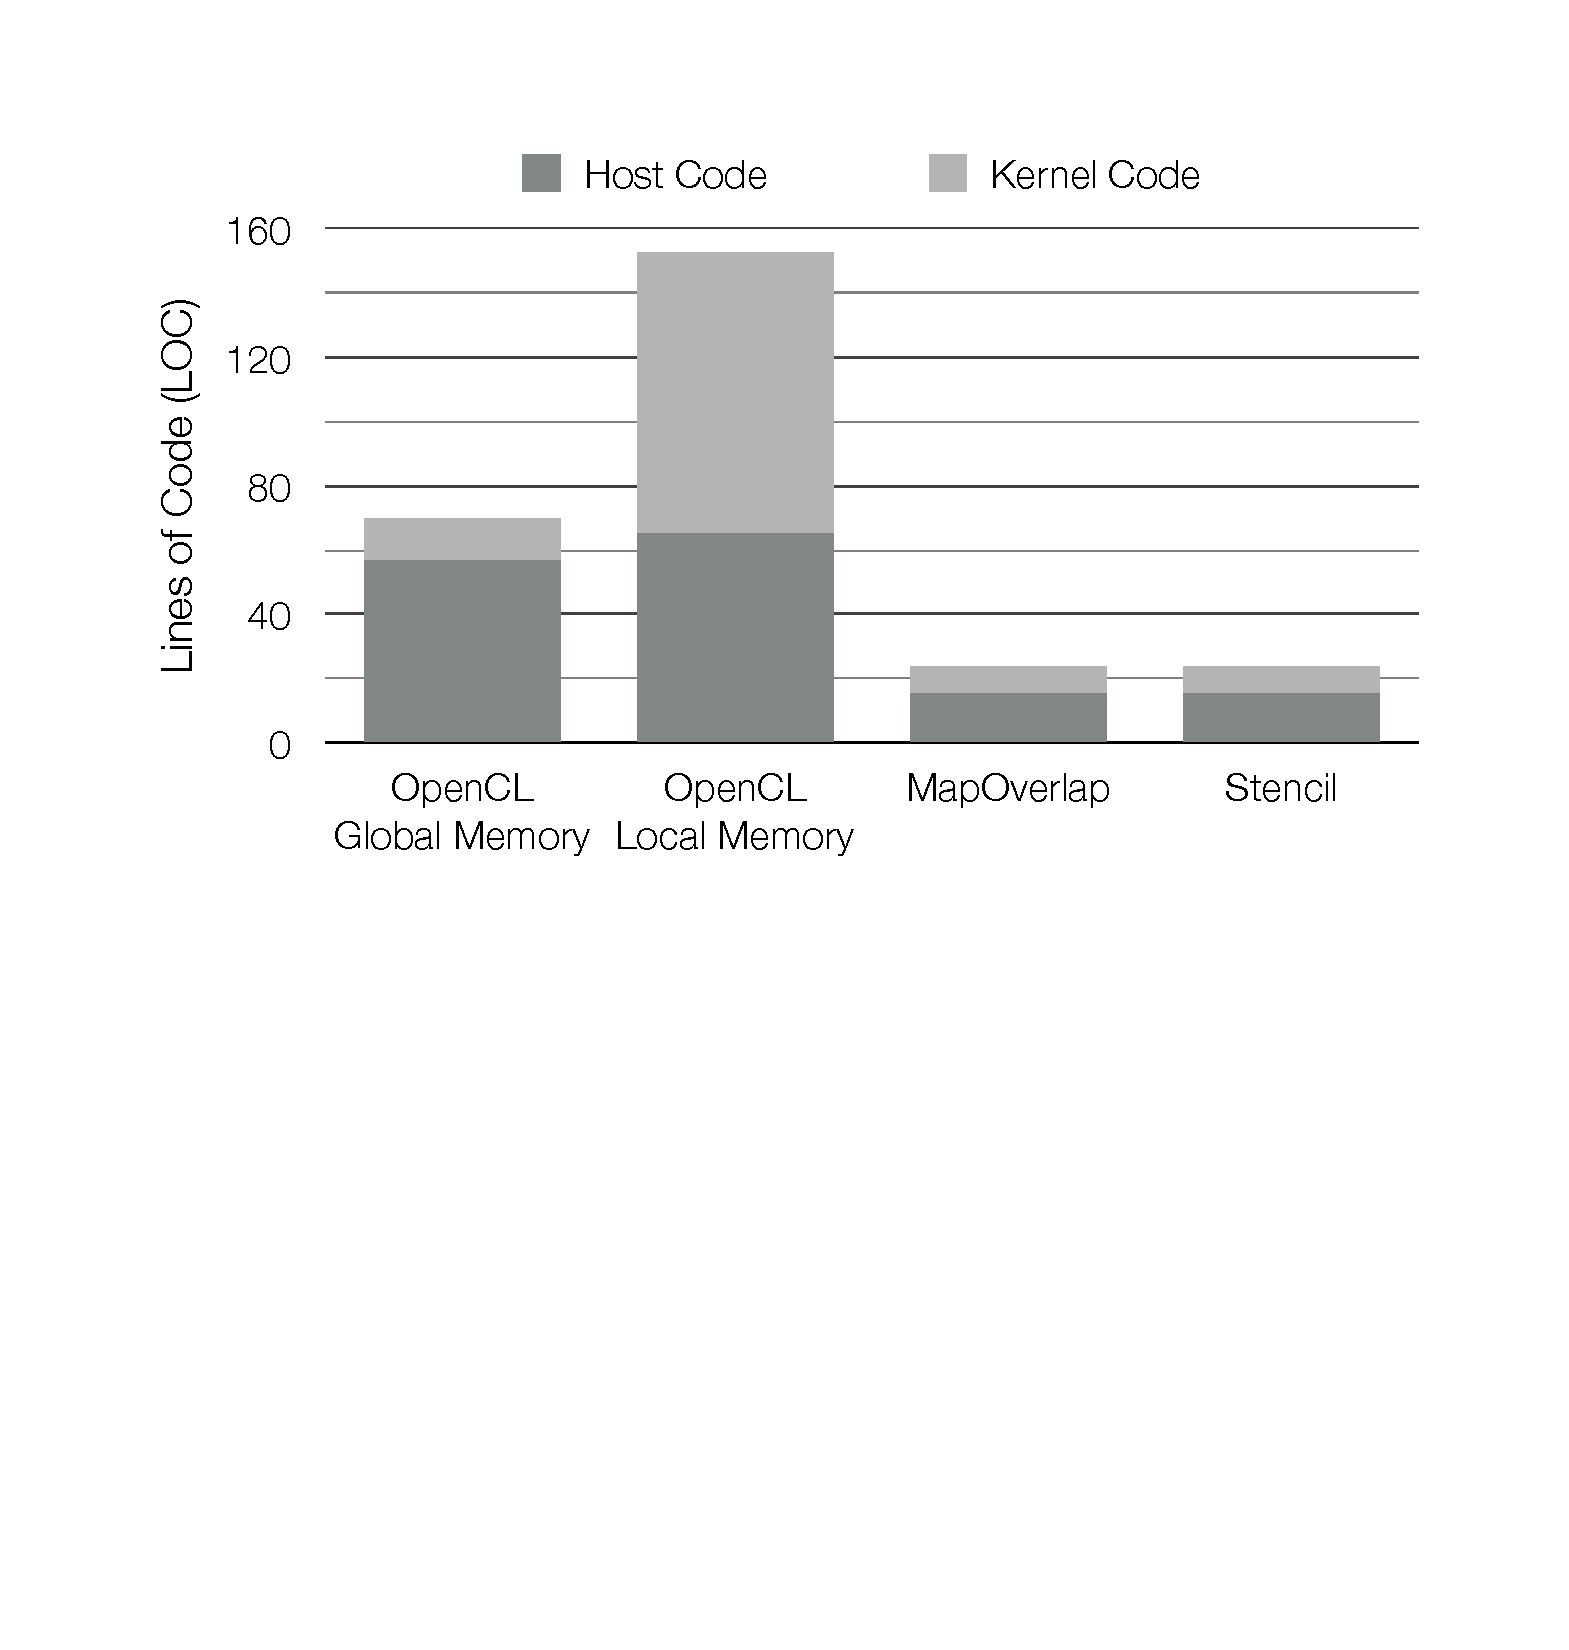
\includegraphics[width=\columnwidth]{HiStencils/LOC.pdf}
	\caption{Lines of code (LOCs) of the Gaussian blur using a na{\"i}ve OpenCL implementation with global memory, an optimized OpenCL version using local memory and SkelCL's MapOverlap and Stencil skeletons.}
	\label{fig:gaussLOCs}
\end{figure} 

Figure~\ref{fig:gaussLOCs} shows the program sizes (in lines of code) for the four implementations. 
The application developer needs $57$ lines of OpenCL host code and 13 LOCs for performing a Gaussian blur with global memory. 
When using local memory, some more arguments are passed to the kernel, increasing the host-LOCs to $65$, while the LOCs for the kernel function, which copies all necessary elements for a work-group's calculation into local memory, requires $88$ LOCs with explicit out-of-bounds handling and complex index calculations.
MapOverlap and Stencil are similar to use and both require only $15$ LOCs host code and $9$ LOCs kernel code to perform a Gaussian blur. 
The support for multi-GPU systems is implicitly given when using SkelCL's skeletons, such that the kernel remains the same as for one-GPU systems.
This is an important advantage of SkelCL over the OpenCL implementations of the Gaussian blur which are single-GPU only, and they require additional LOCs when fitting to multi-GPU environments.

The implementations using MapOverlap and Stencil are only $5-10\%$ slower than an optimized OpenCL implementation of the Gaussian blur while being much shorter than the OpenCL version.

\paragraph{Gaussian Blur using multiple GPUs}

Figure \ref{fig:GaussMult} shows the speedup achieved on the Gaussian blur using \code{Stencil} on up to four devices.
The higher the computational complexity for increasing size of stencil shape, the better the overhead is hidden, leading to a maximum speedup of $1.90$ for two devices, $2.66$ for three devices, and $3.34$ for four devices.
\begin{figure}
	\centering
	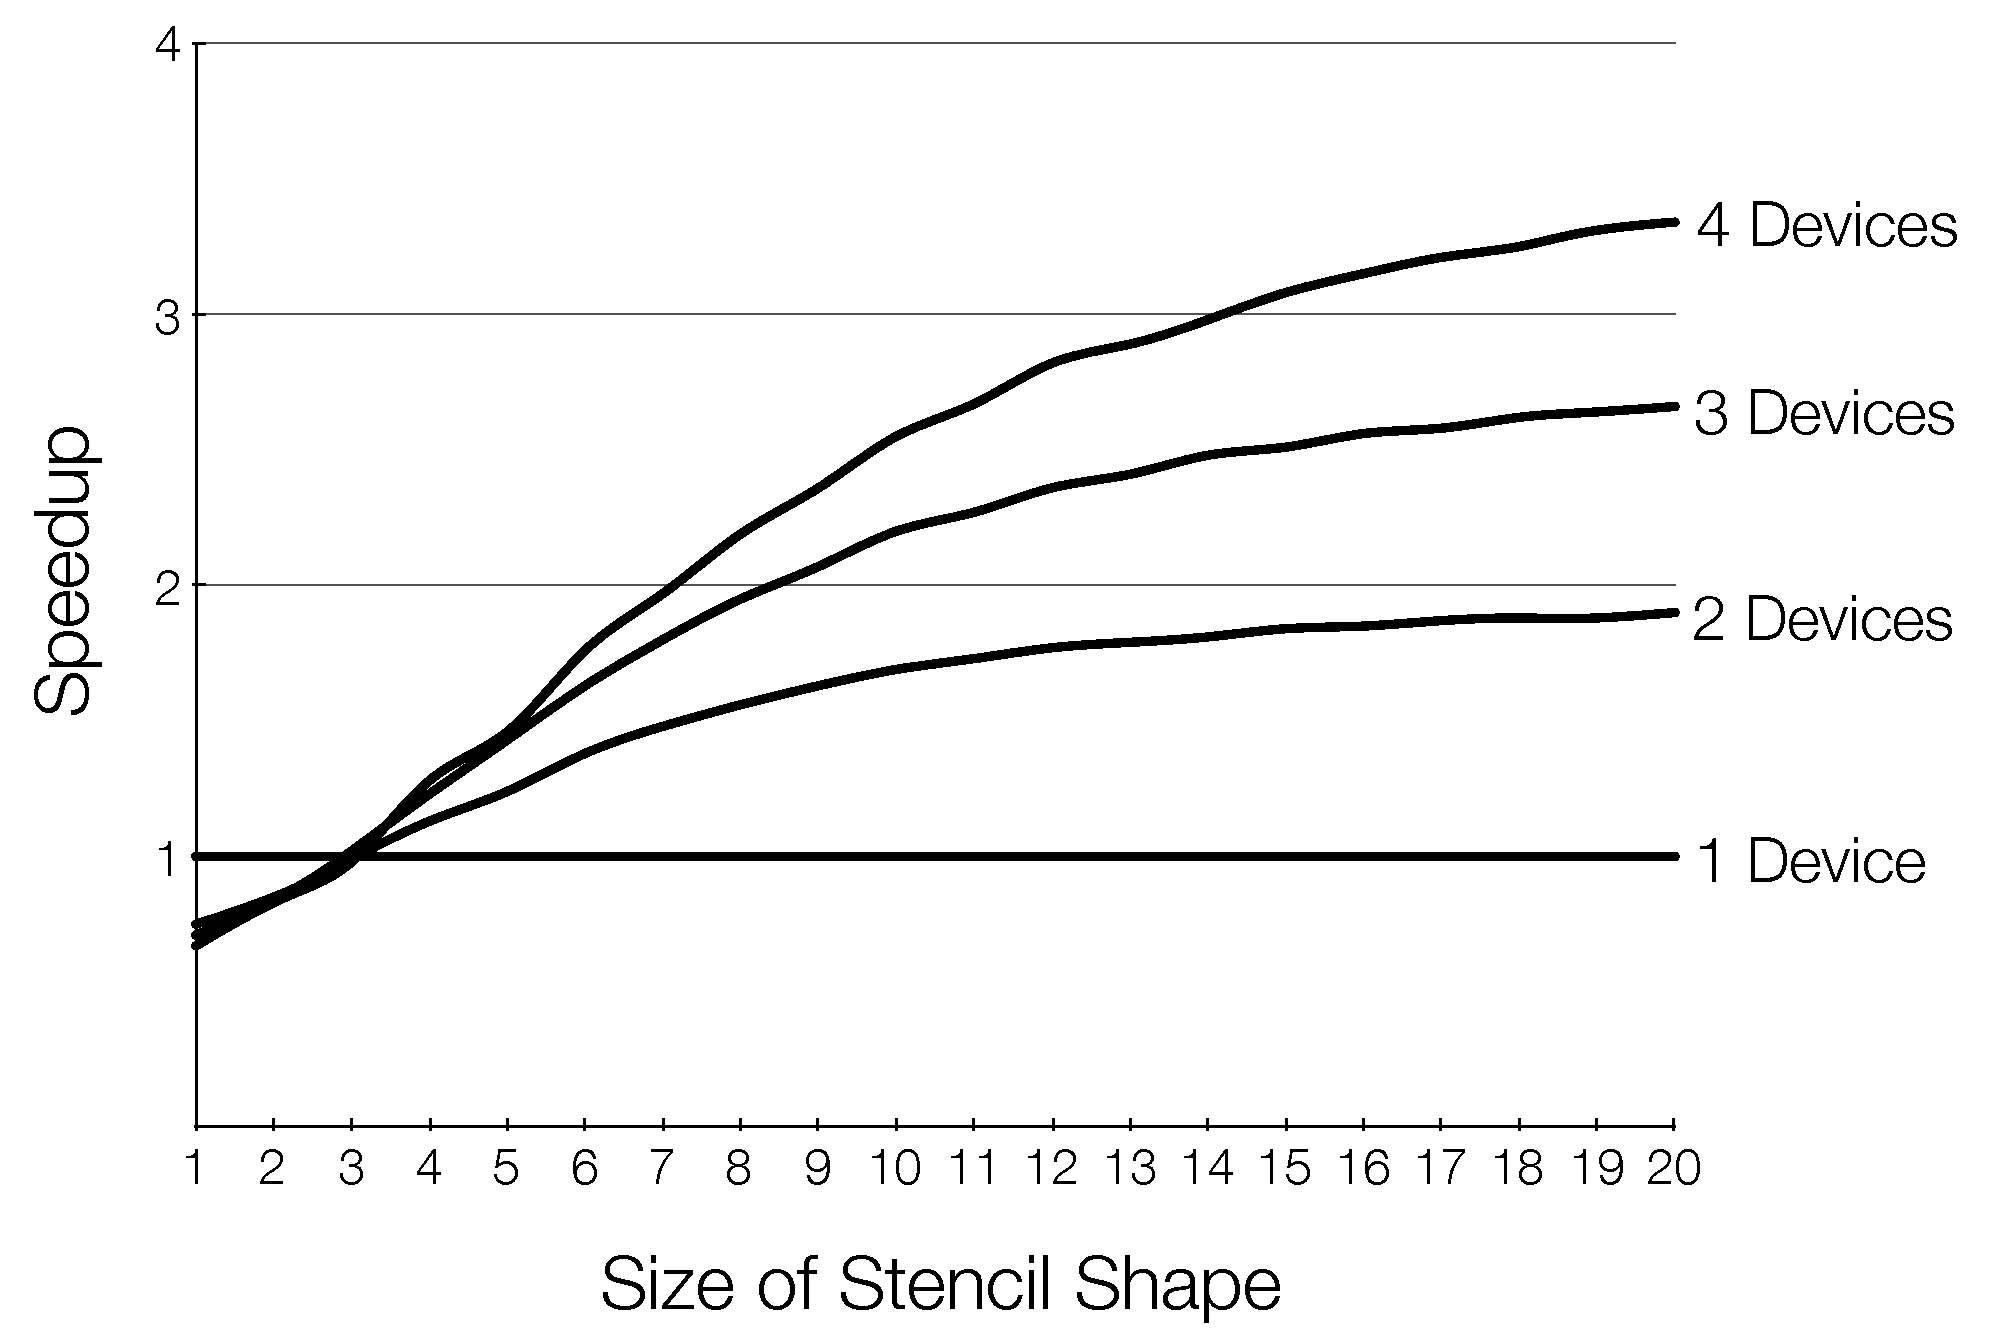
\includegraphics[width=.85\columnwidth]{HiStencils/SpeedupGauss.pdf}
	\caption{Speedup on up to four GPUs.}
	\label{fig:GaussMult}
\end{figure} 
\from{HiStencils end}


\from{Paraphrase begin}
\subsection{Application study: Sobel edge detection (Paraphrase)}
\label{sec:application_study}
To evaluate the  usability and performance of the MapOverlap skeleton and the matrix data type, we implemented an algorithm commonly used in image processing:
The Sobel edge detection is applied to an input image and produces an output image, in which the detected edges in the input image are marked in white and plain areas are shown in black.
Figure~\ref{fig:lena} shows the famous Lena image~\cite{Lena} and the output of Sobel edge detection applied to it.

\begin{figure}[tb]
  \centering
  \begin{subfigure}[t]{.45\textwidth}
    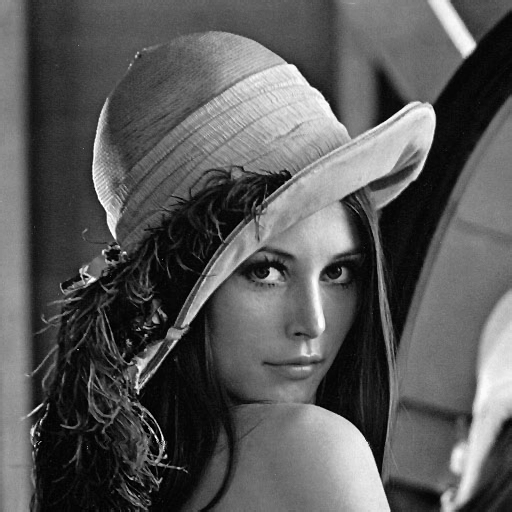
\includegraphics[width=\textwidth]{Paraphrase/lena.png}
    \caption{Original image}
    \label{fig:lena:orig}
  \end{subfigure}
  \hfill
  \begin{subfigure}[t]{.45\textwidth}
    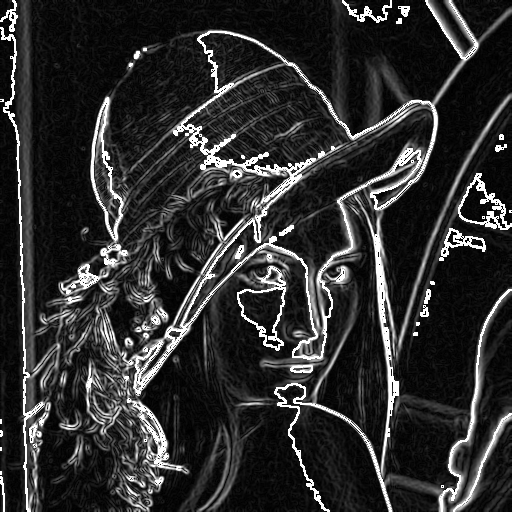
\includegraphics[width=\textwidth]{Paraphrase/sobel_filtered-lena.png}
    \caption{Image after Sobel edge detection}
    \label{fig:lena:sobel}
  \end{subfigure}
  \caption{The famous Lena image often used as an example in image processing.}
  \label{fig:lena}
\end{figure}

Listing~\ref{lst:sobel_seq} shows the algorithm of the Sobel edge detection in pseudo-code.
To keep this version simple, necessary boundary checks are omitted.
In this sequential version, for computing one output value \texttt{out\_img[i][j]} the input value \texttt{img[i][j]} and the direct neighboring elements are needed.
Therefore, the MapOverlap skeleton is a perfect fit for implementing the Sobel edge detection.
\begin{lstlisting}[%
caption={Sequential implementation of the Sobel edge detection.},%
float=tbp,%
label={lst:sobel_seq}]
for (i = 0; i < width; ++i)
  for (j = 0; j < height; ++j)
    h = -1*img[i-1][j-1] +1*img[i+1][j-1]
        -2*img[i-1][j  ] +2*img[i+1][j  ]
        -1*img[i-1][j+1] +1*img[i+1][j+1];
    v = ...;
    out_img[i][j] = sqrt(h*h + v*v);
\end{lstlisting}

Listing~\ref{lst:sobel_skelcl} shows the SkelCL implementation using the MapOverlap skeleton and the matrix type.
The implementation is straightforward and very similar to the sequential version in Listing~\ref{lst:sobel_seq}.
The only notable difference is that for accessing elements the \texttt{get} function is used instead of the square bracket notation.

\begin{lstlisting}[%
caption={SkelCL implementation of the Sobel edge detection.},%
float=tbp,%
label={lst:sobel_skelcl}]
// skeleton customized with Sobel edge detection algorithm
MapOverlap<char(char)> m( "char func(const char* img) {
  short h = -1*get(img,-1,-1) +1*get(img,+1,-1)
            -2*get(img,-1, 0) +2*get(img,+1, 0)
            -1*get(img,-1,+1) +1*get(img,+1,+1);
  short v = ...;
  return sqrt(h*h + v*v); }", 1, SCL_NEUTRAL, 0);
Matrix<char> out_img = m(img); // execution of the skeleton
\end{lstlisting}

Listing~\ref{lst:sobel_opencl} shows a part of the standard OpenCL implementation for Sobel edge detection.
The actual computation is performed inside the \texttt{computeSobel} function, which is omitted in the listing, since it is quite similar to the sequential version describing the actual Sobel edge detection algorithm.
The listing shows that extra low-level code is necessary to deal with technical details, like boundary checks and index calculations.
These extra lines are arguably complex and error-prone because they handle low-level details, rather than the application logic.

\begin{lstlisting}[%
caption={Additional boundary checks and index calculations, necessary in the standard OpenCL implementation.},%
float=tbp,%
label={lst:sobel_opencl}]
__kernel void sobel_kernel( __global const char* img,
                            __global       char* out_img,
                                     int w, int h ) {
 size_t i = get_global_id(0);   size_t j = get_global_id(1);

 if(i < w && j < h) {
  // perform boundary checks
  char ul = (j-1 > 0 && i-1 > 0) ? img[((j-1)*w)+(i-1)] : 0;
  char um = (j-1 > 0           ) ? img[((j-1)*w)+(i+0)] : 0;
  char ur = (j-1 > 0 && i+1 < w) ? img[((j-1)*w)+(i+1)] : 0;
  // ... 5 more
  char lr = (j+1 < h && i+1 < w) ? img[((j+1)*w)+(i+1)] : 0;

  out_img[j * w + i] = computeSobel(ul, um, ur, ..., lr); } }
\end{lstlisting}

We performed runtime experiments using a NVIDIA Tesla T10 GPU with 480 processing elements and 4 GByte memory.
Figure~\ref{fig:measurements} shows the runtime of the OpenCL version in Listing~\ref{lst:sobel_opencl} vs. the SkelCL version with the MapOverlap skeleton in Listing~\ref{lst:sobel_skelcl}.
Only the kernel runtimes are shown, as the data transfer times are equal for both versions.
Measurements were taken using the OpenCL profiling API.
Besides the Lena image~\cite{Lena} with a size of $512\times 512$ pixel, we also used a bigger image by NASA showing the world~\cite{NASA} with a resolution of $15296\times 7648$ pixel.
The mean values of 6 runs are shown in Figure~\ref{fig:measurements}.
The Lena image is shown on the left, the NASA world image on the right.

\begin{figure}[tb]
  \centering
  \begin{subfigure}[t]{.45\textwidth}
    \includegraphics[width=\textwidth]{Paraphrase/lena.pdf}
    \caption{Example image: Lena}
    \label{fig:measurements:lena}
  \end{subfigure}
  \hfill
  \begin{subfigure}[t]{.45\textwidth}
    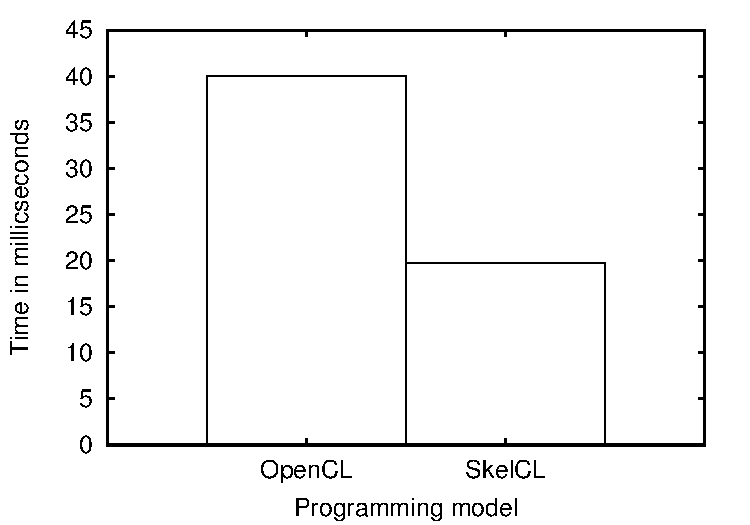
\includegraphics[width=\textwidth]{Paraphrase/world.pdf}
    \caption{Performance results (runtimes)}
    \label{fig:measurements:world}
  \end{subfigure}
  \caption{Performance results (runtimes)}
  \label{fig:measurements}
\end{figure}

The SkelCL version clearly outperforms the OpenCL implementation.
This is due to the fact, that the MapOverlap skeleton uses the fast local memory inside its implementation which is hidden from the application developer.

In addition to the performance advantage, the SkelCL program is also significantly simpler than the cumbersome OpenCL implementation.
The OpenCL implementation requires 19 lines in total while the SkelCL program only comprises 4.
No index calculations or boundary checks are necessary in the SkelCL version whereas they are crucial for a correct implementation in OpenCL.

The OpenCL program in Listing~\ref{lst:sobel_opencl} is not an optimized, but rather a straightforward version most programmers who are not OpenCL experts would write.
Since SkelCL targets such programmers rather than GPU experts, we take this version for comparison with the SkelCL version.
An optimized OpenCL version, e.g., using local memory would probably perform better but would definitely require additional low-level code.
\from{Paraphrase end}

\from{PaCT begin}
\subsection{Application Study: Sobel Edge Detection (PaCT)}
\label{sec:application_study}
To evaluate the  usability and performance of the MapOverlap skeleton on the matrix data type, we implemented the Sobel edge detection that produces an output image in which the detected edges in the input image are marked in white and plain areas are shown in black.

\bigskip
\begin{lstlisting}[%
caption={Sequential implementation of the Sobel edge detection.},%
label={lst:sobel_seq}]
for (i = 0; i < width; ++i)
  for (j = 0; j < height; ++j)
    h = -1*img[i-1][j-1] +1*img[i+1][j-1]
        -2*img[i-1][j  ] +2*img[i+1][j  ]
        -1*img[i-1][j+1] +1*img[i+1][j+1];
    v = ...;
    out_img[i][j] = sqrt(h*h + v*v);
\end{lstlisting}
\bigskip

Listing~\ref{lst:sobel_seq} shows the algorithm of the Sobel edge detection in pseudo-code, with omitted boundary checks for brevity.
In this sequential version, for computing an output value \texttt{out\_img[i][j]} the input value \texttt{img[i][j]} and the direct neighboring elements are needed.
Therefore, the MapOverlap skeleton is a perfect fit for implementing the Sobel edge detection.

\bigskip
\begin{lstlisting}[%
caption={SkelCL implementation of the Sobel edge detection.},%
label={lst:sobel_skelcl}]
// skeleton customized with Sobel edge detection algorithm
MapOverlap<char(char)> m( "char func(const char* img) {
  short h = -1*get(img,-1,-1) +1*get(img,+1,-1)
            -2*get(img,-1, 0) +2*get(img,+1, 0)
            -1*get(img,-1,+1) +1*get(img,+1,+1);
  short v = ...;
  return sqrt(h*h + v*v); }", 1, SCL_NEUTRAL, 0);
Matrix<char> out_img = m(img); // execution of the skeleton
\end{lstlisting}
\bigskip

Listing~\ref{lst:sobel_skelcl} shows the SkelCL implementation using the MapOverlap skeleton and the matrix data type.
The implementation is straightforward and very similar to the sequential version in Listing~\ref{lst:sobel_seq}.
The only notable difference is that for accessing elements the \texttt{get} function is used instead of the square bracket notation.

\bigskip
\begin{lstlisting}[%
caption={Additional boundary checks and index calculations for Sobel algorithm, necessary in the standard OpenCL implementation.},%
label={lst:sobel_opencl}]
__kernel void sobel_kernel( __global const uchar* img,
                            __global       uchar* out_img)
 uint i = get_global_id(0);   uint j = get_global_id(1);
 uint w = get_global_size(0); uint h = get_global_size(1);
 // perform boundary checks
 if(i >= 1 && i < (w-1) && j >= 1 && j < (h-1)) {
  char ul = img[((j-1)*w)+(i-1)];
  char um = img[((j-1)*w)+(i+0)];
  char ur = img[((j-1)*w)+(i+1)];
  // ... 5 more
  char lr = img[((j+1)*w)+(i+1)];

  out_img[j * w + i] = computeSobel(ul, um, ur, ..., lr); } }
\end{lstlisting}
\bigskip


Listing~\ref{lst:sobel_opencl} shows a part of the OpenCL implementation for Sobel edge detection provided by AMD as an example for their software development kit~\cite{AMDSDK-13}.
The actual computation is performed inside the \texttt{computeSobel} function, which is omitted in the listing, since it is quite similar to the sequential version in Listing~\ref{lst:sobel_seq}.
The listing shows that extra low-level code is necessary to deal with technical details, like boundary checks and index calculations, which are arguably complex and error-prone.

\begin{figure}[tbp]
  \vspace{.5em}
  \centering
  \includegraphics[height=4.5cm]{PaCT/lena.pdf}
  \caption{Performance results for Sobel edge detection}
  \label{fig:measurements}
  \vspace{-1em}
\end{figure}
We performed runtime experiments using one NVIDIA Tesla GPU with 480 processing elements and 4 GByte memory.
Figure~\ref{fig:measurements} shows the runtime of two OpenCL versions (from AMD and NVIDIA SDK) vs. the SkelCL version with the MapOverlap skeleton presented in Listing~\ref{lst:sobel_skelcl}.
Only the kernel runtimes are shown, as the data transfer times are equal for all versions.
Measurements were taken using the OpenCL profiling API.
We used the popular Lena image~\cite{Lena} with a size of $512\times 512$ pixel and took the mean values of six runs.
The AMD version is clearly slower then the two other implementations, because it does not use the fast local memory which the NVIDIA implementation and the MapOverlap skeleton of SkelCL do.
SkelCL totally hides the memory management details inside its implementation from the application developer.
The NVIDIA and SkelCL implementations perform similar.
In this particular example, SkelCL even slightly outperforms the implementation by NVIDIA.

In addition to the performance advantage over the AMD and NVIDIA versions, the SkelCL program is also significantly simpler than the cumbersome OpenCL implementation.
The SkelCL program only comprises the few lines of code shown in Listing~\ref{lst:sobel_skelcl}.
The AMD implementations requires 37 lines of code for its kernel implementation and the NVIDIA implementation requires even 208 lines of code.
Both versions require additional lines of code for the host program which manages the execution of the OpenCL kernel.
No index calculations or boundary checks are necessary in the SkelCL version whereas they are crucial for a correct implementation in OpenCL.
\from{PaCT end}


\from{HiStencils begin}
\subsection{Canny Edge Detection (HiStencils)}
\begin{figure}[tbp]
	\centering
	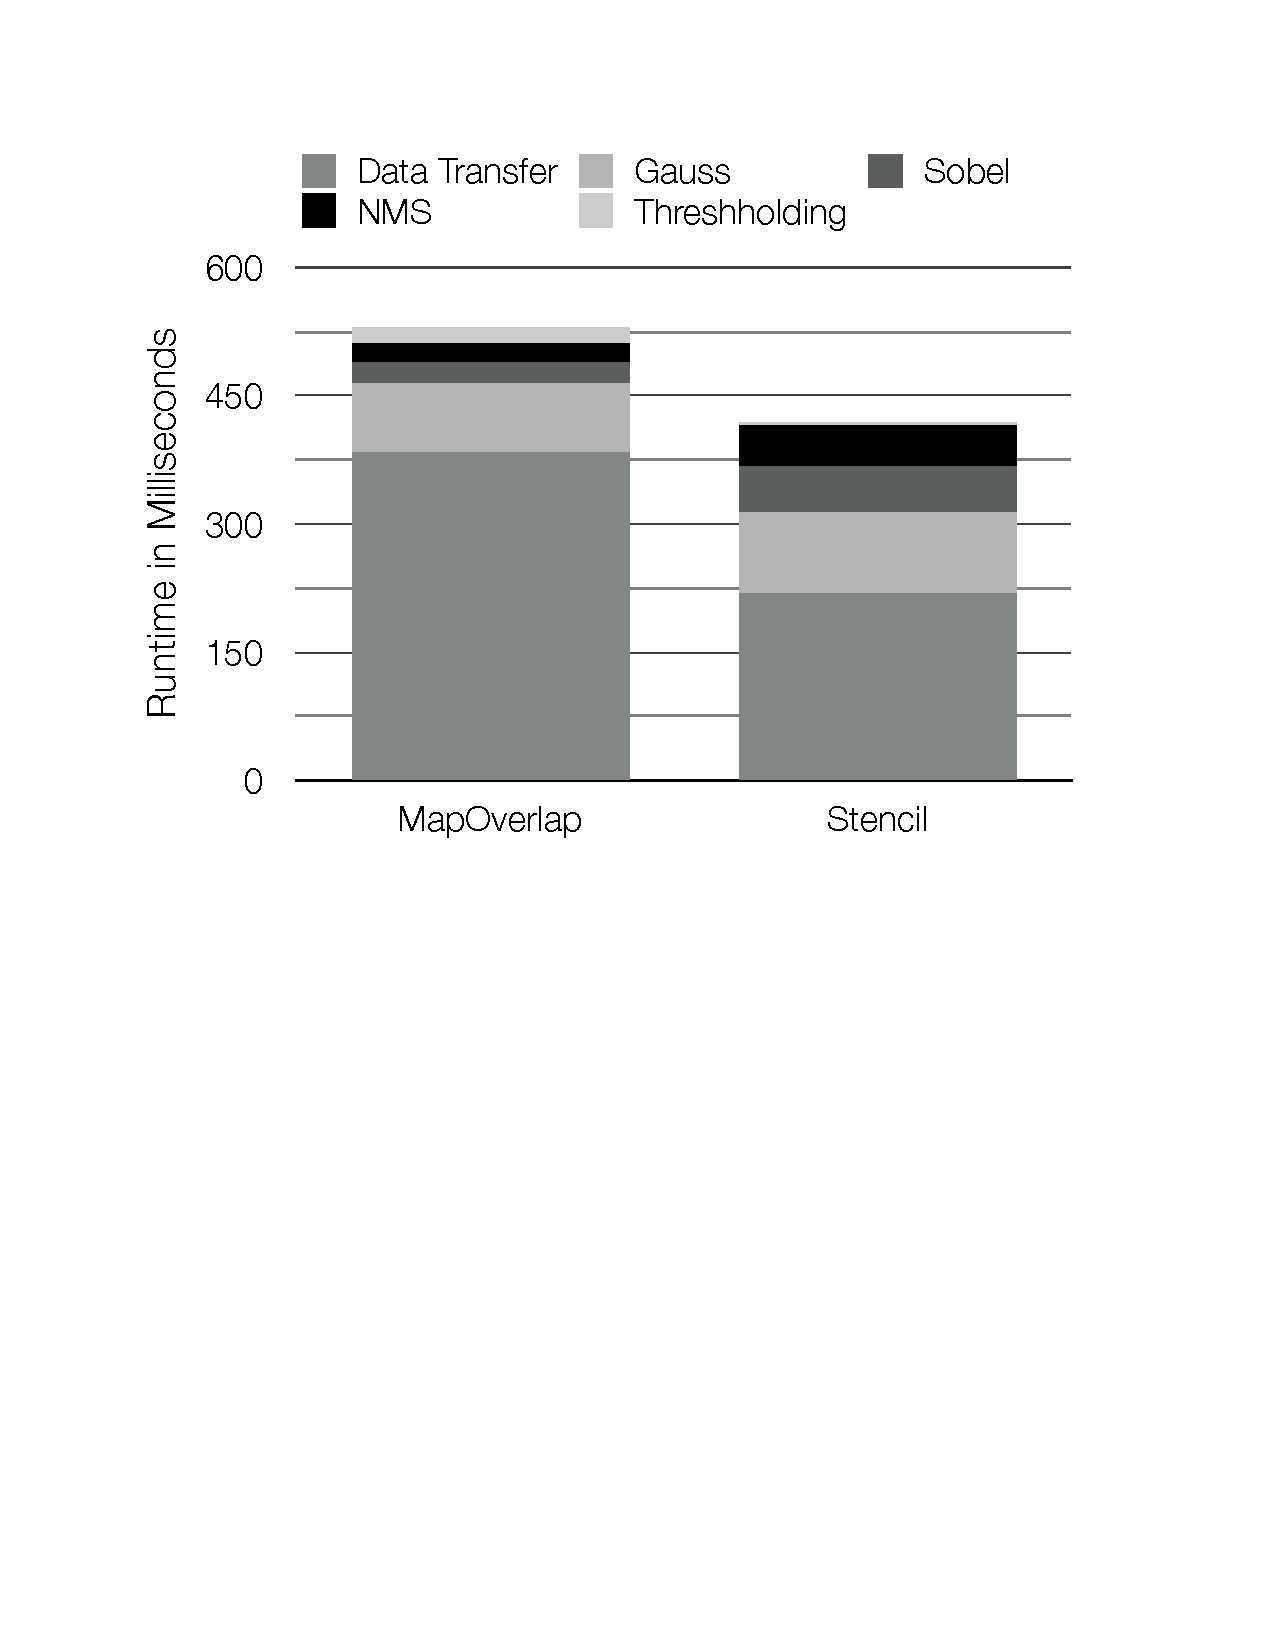
\includegraphics[width=.9\columnwidth]{HiStencils/Canny.pdf}
	\caption{Runtime of the Canny algorithm implemented with the MapOverlap and Stencil skeletons.}
	\label{fig:canny}
\end{figure} 

Figure~\ref{fig:canny} shows the absolute runtime of the Canny algorithm (Listing \ref{lst:canny01}). 
As the MapOverlap skeleton appends padding elements to the matrix, the matrix has to be downloaded, resized and uploaded again to the GPU between each step of the sequence.
This additional work to an increased time for data transfers. 
The Gaussian blur with a stencil shape extent of $2$, as well as the Sobel filter and the non-maximum suppression with a stencil shape of $1$, are $2.1$ to $2.2$ times faster when using MapOverlap. 
However, the threshold operation, which is expressed as the Map skeleton in the Stencil sequence, is $6.8$ times faster than MapOverlap's threshold operation.
Overall, when performing sequences of stencil operations, the Stencil skeleton reduces the number of copy operations and therefore leads to a better overall performance.
When performing the Canny algorithm, Stencil outperforms MapOverlap by $21\%$.
\from{HiStencils end}


\begin{lstlisting}[%
caption={MapOverlap skeleton computing the sum of all direct neightbors for every element in a matrix},%
float=tbp,%
label={lst:mapoverlap01}]
MapOverlap<float(float)> m("float func(float* m_in){
     float sum = 0.0f;
     for (int i = -1; i < 1; ++i)
       for (int j = -1; j < 1; ++i)
         sum += get(m_in, i, j);
     return sum;
   }", 1, SCL_NEUTRAL, 0.0f);
\end{lstlisting}

Listing~\ref{lst:raw_opencl01} shows how the same simple calculation can be performed in standard OpenCL.
While the amount of lines of code increases by a factor of 2, the complexity of each single line also increases, as follows.
Besides a pointer to the output memory, the width of the matrix has to be provided as parameter.
The correct index has to be calculated for every memory access using an offset and the width of the matrix.
Therefore, knowledge about how the two-dimensional matrix is stored in one-dimensional memory is required.
In addition, manual boundary checks have to be performed to avoid faulty memory accesses.\bigskip

\begin{lstlisting}[%
caption={An OpenCL kernel performing the same calculation as the MapOverlap skeleton shown in Listing~\ref{lst:mapoverlap01}.\bigskip},%
label={lst:raw_opencl01}]
__kernel void sum_up(__global float* m_in,
                     __global float* m_out,
                     int width, int height) {
  int i_off = get_global_id(0); int j_off = get_global_id(1);
  float sum = 0.0f;
  for (int i = i_off - 1; i < i_off + 1; ++i)
    for (int j = j_off - 1; j < j_off + 1; ++j) {
      // perform boundary checks
      if ( i < 0 || i > width || j < 0 || j > height )
        continue;
      sum += m_in[ j * width + i ];     }
  m_out[ j_off * width + i_off ] = sum; }
\end{lstlisting}

SkelCL avoids all these low-level details.
Neither additional parameter, nor index calculations or manual boundary checks are necessary.
In SkelCL, the application developer only provides the source code implementing the steps required by the algorithm.


In the actual source code, the application developer provides the function $f$ which receives a pointer to the element in the middle, $m_{in}[i,j]$.

\begin{lstlisting}[%
caption={MapOverlap skeleton computing the sum of all direct neightbors for every element in a matrix},%
float=bp,%
label={lst:mapoverlap01}]
MapOverlap<float(float)> m("float func(float* m_in){
float sum = 0.0f;
for (int i = -1; i < 1; ++i)
  for (int j = -1; j < 1; ++i)
    sum += get(m_in, i, j); return sum;
}", 1, SCL_NEUTRAL, 0.0f);
\end{lstlisting}


Listing~\ref{lst:mapoverlap01} shows a simple example of computing the sum of all direct neighboring values using the MapOverlap skeleton.
To access the elements of the input matrix $m_{in}$, function \texttt{get} is provided by SkelCL.
All indices are specified relative to the middle element $m_{in}[i,j]$; therefore, for accessing this element the function call \texttt{get(m\_in, 0, 0)} is used.
The application developer must ensure that only elements in the range specified by the second argument $d$ of the MapOverlap skeleton, are accessed.
In Listing~\ref{lst:mapoverlap01}, range is specified as $d=1$, therefore, only direct neighboring elements are accessed.
To enforce this property, boundary checks are performed at runtime by the \texttt{get} function.
In future work, we plan to avoid boundary checks at runtime by statically proving that all memory accesses are in bounds, as it is the case in the shown example.

\begin{lstlisting}[%
caption={An OpenCL kernel performing the same calculation as the MapOverlap skeleton shown in Listing~\ref{lst:mapoverlap01}.},%
float=tbp,%
label={lst:raw_opencl01}]
__kernel void sum_up(__global float* m_in,
                     __global float* m_out,
                     int width, int height) {
  int i_off = get_global_id(0); 
  int j_off = get_global_id(1);
  float sum = 0.0f;
  for (int i = i_off - 1; i < i_off + 1; ++i)
    for (int j = j_off - 1; j < j_off + 1; ++j) {
      // perform boundary checks
      if ( i < 0 || i > width || j < 0 || j > height )
        continue;
      sum += m_in[ j * width + i ];     }
  m_out[ j_off * width + i_off ] = sum; }
\end{lstlisting}


Listing~\ref{lst:raw_opencl01} shows how the same simple calculation can be performed in standard OpenCL.
While the amount of lines of code increases by a factor of 2, the complexity of each single line also increases:
1) Besides a pointer to the output memory, the width of the matrix has to be provided as parameter; 2) the correct index has to be calculated for every memory access using an offset and the width of the matrix, i.\,e.
knowledge about how the two-dimensional matrix is stored in one-dimensional memory is required.
3) In addition, manual boundary checks have to be performed to avoid faulty memory accesses. 

SkelCL avoids all these low-level details.
Neither additional parameter, nor index calculations or manual boundary checks are necessary.

\from{HiStencils}
Listing~\ref{lst:mapoverlap01} shows the implementation of the Sobel edge detection using the \emph{MapOverlap} skeleton.
The MapOverlap skeleton applies a given function $func$ (defined in lines 2--6) to each element of an input matrix $in_{img}$ while taking the neighboring elements within the range $[-d, +d]$ in each dimension into account.
Here, $d$ is the second parameter (line 7) and two additional parameters define how the skeleton handles out-of-bound memory accesses (line 8).
A helper function (\code{get}) is used to easily access the neighboring elements.
The indexes are specified relative to the current element, e.\,g. to access the element on the left the function call \code{get(in, -1, 0)} is used.

Special handling is necessary when accessing elements out of the boundaries of the matrix, e.g., when the item in the top-left corner of the matrix accesses elements above and left of it.
The MapOverlap skeleton can be configured to handle such out-of-bound memory accesses in two possible ways:
1) a specified neutral value is returned;
2) the nearest valid value inside the matrix is returned.
In Listing~\ref{lst:mapoverlap01}, the first option is chosen and $0$ is provided as neutral value.

\begin{lstlisting}[%
caption={Implementation of Sobel edge detection using the MapOverlap skeleton},%
float=tbp,%
label={lst:mapoverlap01}]
MapOverlap<char(char)> sobel(
 "char func(const char* in_img) {
    char ul = get(in_img, -1, -1);
    ...
    char lr = get(in_img, +1, +1);
    return computeSobel(ul,..., lr);}",
 1, Padding::NEUTRAL, 0);

output = sobel(input);
\end{lstlisting}

Simple stencil computations with a regular stencil shape can easily be expressed using the MapOverlap skeleton.
For more complex stencil computations, e.\,g. iterative stencils, we introduce the more advanced \emph{Stencil} skeleton.

\paragraph{The MapOverlap Skeleton}

Listing~\ref{lst:stencil01} shows the implementation of an iterative stencil application simulating heat transfer.
This application simulates heat spreading from one location and flowing throughout a two-dimensional simulation space.
\begin{lstlisting}[%
caption={Implementation of heat simulation using the Stencil skeleton},%
float=tbp,%
label={lst:stencil01}]
Stencil<char(char)> heatSim(
 "char func(const char* in) {
    char lt = get(in, -1, -1);
    char lm = get(in, -1,  0);
    char lb = get(in, -1, +1);
    return computeHeat(lt, lm, lb); }",
 StencilShape(1, 0, 1, 1),
 Padding::NEUTRAL, 255);

output = heatSim(100, input);
\end{lstlisting}


The application developer specifies the function (line 2--6) describing the computation and, therefore, the stencil shape, as well as the stencil shape's extents (line 7) and the out-of-bound handling (line 8).
The stencil shape's extents are specified using four values for each of the directions:
up, right, down, left.
In the example in Listing~\ref{lst:stencil01}, the heat flows from left to right, therefore, no accesses to elements to the right are necessary and the stencil space's extents are specified accordingly (note the $0$ in line 7 representing the extent to the right).
Figure~\ref{fig:stencilShape} illustrates this situation: the dark gray element is updated by using the values from the left.
The specified stencil shape's extent is highlighted in light gray.
In our current implementation, the user has to explicitly specify the stencil shape's extents, which is necessary for performing the out-of-bound handling on the GPU.
In future work, we plan to automatically infer the stencil shape's extents
from the customizing function using source code analysis in order to free the user from specifying this information explicitly.
\begin{figure}
  \begin{centering}
    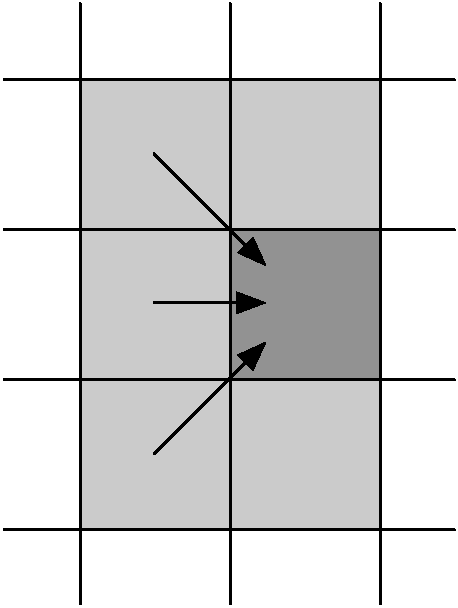
\includegraphics[width=.18\textwidth]{HiStencils/heat_transfer}
    \caption{Stencil shape for heat transfer simulation}
    \label{fig:stencilShape}
    \vspace{-.5em}
  \end{centering}
\end{figure}

Many stencil applications apply a stencil multiple times for a fixed number of iterations, or until a certain condition is met.
For example, to iterate the heat transfer simulation for one hundred steps, we specify the number of iterations to perform when executing the skeleton (line 10).
In the future, we plan to allow the user to specify a custom function which checks a condition to stop the iterations.

The MapOverlap skeleton can be configured to handle out-of-bounds accesses by returning the nearest valid value of the input matrix.
Another distinction can be made regarding iterations and sequences of stencil operations:
using elements of the \textbf{initial}, user-provided input matrix or using elements of the \textbf{current} step's input matrix, which already was updated during earlier stencil operations.
The Stencil skeleton can be configured to handle out-of-bounds accesses in both ways, thus offering three possible ways, including the neutral value. 
For each of them, there is an own kernel function, loading appropriate elements into local memory. 






Simple stencil computations with a regular stencil shape can easily be expressed using the \mapOverlap skeleton.
For more complex stencil computations, \eg iterative stencil computations, we introduce the more advanced \stencil skeleton.





Real-world applications often perform multiple stencil operations in sequence.
Let us consider the popular \emph{Canny algorithm} which is used for detecting edges in images.
For the sake of simplicity we consider a simplified version, which applies the following stencil operations in a sequence:
1), a noise reduction operation is applied, e.g., a Gaussian filter;
2), an edge detection operator like the Sobel filter is applied;
3), the so-called non-maximum suppression is performed, where all pixels in the image are colored black except pixels being a local maximum;
4), a threshold operation is applied to produce the final result.
A more complex version of the algorithm performs the edge tracking by hysteresis, as an additional step.
This results in detecting some weaker edges, but even without this additional step the algorithm usually achieves good results.

In SkelCL, each single step of the Canny algorithm can be expressed using the Stencil skeleton.
The last step, threshold operation, does not need access to neighboring elements, as the user threshold function only checks the value of the current pixel.
Therefore, this step can be expressed using SkelCL's simpler Map skeleton.
The Stencil skeleton's implementation automatically uses the simpler Map skeleton's implementation when the user specifies a stencil shape which extents are $0$ in all directions.

\begin{lstlisting}[%
  caption={Structure of the Canny algorithm as implemented with a sequence of skeletons.},%
  float=tbp,%
  label={lst:canny01}]
Stencil<Pixel(Pixel)> gauss(...);
Stencil<Pixel(Pixel)> sobel(...);
Stencil<Pixel(Pixel)> nms(...);
Stencil<Pixel(Pixel)> threshold(...);

StencilSequence<Pixel(Pixel)> canny(
  gauss, sobel, nms, threshold);

output = canny(1, input);
\end{lstlisting}

To implement the Canny algorithm in SkelCL, the single steps can be combined as shown in Listing~\ref{lst:canny01}.
The individual steps are defined in lines 1--4 and then combined to a sequence of stencils in line 6 and 7.
During execution (line 9), the stencil operation are performed in the order which is specified when creating the \emph{StencilSequence} object.

